\chapter{图}

\section{图}

\subsection{图(Graph)}

你的微信中有若干好友,而你的好友又有若干好友。许许多多的用户组成了一个多对多的关系网,这个关系网就是数据结构中的图。\\

再例如使用地图导航功能时,导航会根据你的出发地和目的地规划最佳的地铁换乘路线。许许多多的地铁站组成的交通网络也可以认为是图。\\

图是一种比树更为复杂的数据结构。树的结点之间是一对多的关系,并且存在父与子的层级划分。而图的顶点之间是多对多关系,并且所有顶点都是平等的,无所谓谁是父子。\\

在图中,最基本的单元是顶点(vertex),相当于树中的结点。顶点之间的关联关系被称为边(edge)。图中包含一组顶点和一组边,通常用V表示顶点集合,用E表示边集合。边可以看作是顶点对,即$ (v, w) \in E,\ v, w \in V $。\\

在有些图中,每一条边并不是完全等同的。例如地铁线路,站与站之间的距离都有可能不同。因此图中会涉及边的权重(weight),涉及到权重的图被称为带权图(weighted graph),也称为网络。

\begin{figure}[H]
	\centering
	\begin{tikzpicture}
		\begin{scope}[every node/.style={circle,thick,draw}]
			\node (A) at (0,0) {A};
			\node (B) at (0,3) {B};
			\node (C) at (2.5,4) {C};
			\node (D) at (2.5,1) {D};
			\node (E) at (2.5,-3) {E};
			\node (F) at (5,3) {F};
		\end{scope}

		\begin{scope}[>={Stealth[black]},
			every node/.style={fill=white,circle},
			every edge/.style={draw=black,very thick}]
			\path [-] (A) edge node {5} (B);
			\path [-] (B) edge node {3} (C);
			\path [-] (A) edge node {4} (D);
			\path [-] (D) edge node {3} (C);
			\path [-] (A) edge node {3} (E);
			\path [-] (D) edge node {3} (E);
			\path [-] (D) edge node {3} (F);
			\path [-] (C) edge node {5} (F);
			\path [-] (E) edge node {8} (F);
		\end{scope}
	\end{tikzpicture}
	\caption{带权图}
\end{figure}

还有一种图,顶点之间的关联并不是完全对称的。拿微信举例,你的好友列表里有我,但我的好友列表里未必有你。\\

这样一来,顶点之间的边就有了方向的区分,这种带有方向的图被称为有向图(directed graph)。有向边可以使用<v, w>表示从v指向w的边。\\

\begin{figure}[H]
	\centering
	\begin{tikzpicture}
		\begin{scope}[every node/.style={circle,thick,draw}]
			\node (A) at (0,0) {A};
			\node (B) at (0,3) {B};
			\node (C) at (2.5,4) {C};
			\node (D) at (2.5,1) {D};
			\node (E) at (5,0) {E};
		\end{scope}

		\begin{scope}[>={Stealth[black]},
			every node/.style={fill=white,circle},
			every edge/.style={draw=black,very thick}]
			\path [<->] (A) edge node {5} (B);
			\path [->] (B) edge node {3} (C);
			\path [->] (A) edge node {4} (D);
			\path [<->] (D) edge node {3} (C);
			\path [<->] (A) edge node {3} (E);
			\path [->] (D) edge node {3} (E);
		\end{scope}
	\end{tikzpicture}
	\caption{有向图}
\end{figure}

相应地,在QQ中,只要我把你从好友里删除,你在自己的好友列表里就看不到我了。因此QQ的好友关系可以认为是一个没有方向区分的图,这种图被称为无向图(undirected graph)。

\newpage

\section{图的表示}

\subsection{邻接矩阵(Adjacency Matrix)}

拥有n个顶点的图,它所包含的边的数量最多是n(n-1)条,因此,要表达各个顶点之间的关联关系,最清晰易懂的方式是使用邻接矩阵G[N][N]。\\

对于无向图来说,如果顶点之间有关联,那么邻接矩阵中对应的值为1;如果顶点之间没有关联,那么邻接矩阵中对应的值为0。

\vspace{-0.5cm}

\begin{align}\nonumber
	G[i][j] = \begin{cases}
		1 & <v_i, v_j>\text{是G中的边}   \\
		0 & <v_i, v_j>\text{不是G中的边} \\
	\end{cases}
\end{align}

\begin{figure}[H]
	\centering
	\begin{tikzpicture}
		\begin{scope}[every node/.style={circle,thick,draw}]
			\node (A) at (0,0) {A};
			\node (B) at (0,3) {B};
			\node (C) at (2.5,4) {C};
			\node (D) at (2.5,1) {D};
			\node (E) at (4,2) {E};
		\end{scope}

		\begin{scope}[>={Stealth[black]},
			every node/.style={},
			every edge/.style={draw=black,very thick}]
			\path [-] (A) edge node {} (B);
			\path [-] (A) edge node {} (D);
			\path [-] (B) edge node {} (C);
			\path [-] (C) edge node {} (D);
			\path [-] (C) edge node {} (E);
		\end{scope}
	\end{tikzpicture}
\end{figure}

\begin{table}[H]
	\centering
	\setlength{\tabcolsep}{5mm}{
		\begin{tabular}{|c|c|c|c|c|c|}
			\hline
			           & \textbf{A} & \textbf{B} & \textbf{C} & \textbf{D} & \textbf{E} \\
			\hline
			\textbf{A} & 0          & 1          & 0          & 1          & 0          \\
			\hline
			\textbf{B} & 1          & 0          & 1          & 0          & 0          \\
			\hline
			\textbf{C} & 0          & 1          & 0          & 1          & 1          \\
			\hline
			\textbf{D} & 1          & 0          & 1          & 0          & 0          \\
			\hline
			\textbf{E} & 0          & 0          & 1          & 0          & 0          \\
			\hline
		\end{tabular}
	}
	\caption{无向图邻接矩阵}
\end{table}

需要注意的是,邻接矩阵从左上到右下的一条对角线上的元素值必然是0,因为任何一个顶点与它自身是没有连接的。同时,无向图对应的邻接矩阵是一个对称矩阵,假如A和B有关联,那么B和A也必定有关联。\\

但是对于有向图的邻接矩阵,不一定是一个对称矩阵,假如A可以达到B,从B未必能达到A。\\

\begin{figure}[H]
	\centering
	\begin{tikzpicture}
		\begin{scope}[every node/.style={circle,thick,draw}]
			\node (A) at (0,0) {A};
			\node (B) at (0,3) {B};
			\node (C) at (2.5,4) {C};
			\node (D) at (2.5,1) {D};
		\end{scope}

		\begin{scope}[>={Stealth[black]},
			every node/.style={},
			every edge/.style={draw=black,very thick}]
			\path [->] (A) edge node {} (B);
			\path [->] (A) edge node {} (C);
			\path [<->] (C) edge node {} (D);
			\path [->] (D) edge node {} (B);
		\end{scope}
	\end{tikzpicture}
\end{figure}

\begin{table}[H]
	\centering
	\setlength{\tabcolsep}{5mm}{
		\begin{tabular}{|c|c|c|c|c|}
			\hline
			           & \textbf{A} & \textbf{B} & \textbf{C} & \textbf{D} \\
			\hline
			\textbf{A} & 0          & 1          & 1          & 0          \\
			\hline
			\textbf{B} & 0          & 0          & 0          & 0          \\
			\hline
			\textbf{C} & 0          & 0          & 0          & 1          \\
			\hline
			\textbf{D} & 0          & 1          & 1          & 0          \\
			\hline
		\end{tabular}
	}
	\caption{有向图邻接矩阵}
\end{table}

对于网络,只要把邻接矩阵对应位置的值定义为边$ <v_i, v_j> $的权重即可。\\

\begin{figure}[H]
	\centering
	\begin{tikzpicture}
		\begin{scope}[every node/.style={circle,thick,draw}]
			\node (A) at (0,0) {A};
			\node (B) at (3,0) {B};
			\node (C) at (5,2.5) {C};
			\node (D) at (1.5,5) {D};
			\node (E) at (-2,2.5) {E};
			\node (F) at (1.5,2.5) {F};
		\end{scope}

		\begin{scope}[>={Stealth[black]},
			every node/.style={fill=white,circle},
			every edge/.style={draw=black,very thick}]
			\path [->] (A) edge node {5} (B);
			\path [->] (A) edge node {2} (F);
			\path [->] (B) edge node {4} (C);
			\path [->] (C) edge node {9} (D);
			\path [->] (D) edge node {7} (E);
			\path [->] (D) edge node {3} (F);
			\path [->] (E) edge node {1} (A);
			\path [->] (F) edge node {1} (C);
			\path [->] (F) edge node {8} (E);
		\end{scope}
	\end{tikzpicture}
\end{figure}

\begin{table}[H]
	\centering
	\setlength{\tabcolsep}{5mm}{
		\begin{tabular}{|c|c|c|c|c|c|c|}
			\hline
			           & \textbf{A} & \textbf{B} & \textbf{C} & \textbf{D} & \textbf{E} & \textbf{F} \\
			\hline
			\textbf{A} & $ \infty $ & 5          & $ \infty $ & $ \infty $ & $ \infty $ & 2          \\
			\hline
			\textbf{B} & $ \infty $ & $ \infty $ & 4          & $ \infty $ & $ \infty $ & $ \infty $ \\
			\hline
			\textbf{C} & $ \infty $ & $ \infty $ & $ \infty $ & 9          & $ \infty $ & $ \infty $ \\
			\hline
			\textbf{D} & $ \infty $ & $ \infty $ & $ \infty $ & $ \infty $ & 7          & 3          \\
			\hline
			\textbf{E} & 1          & $ \infty $ & $ \infty $ & $ \infty $ & $ \infty $ & $ \infty $ \\
			\hline
			\textbf{F} & $ \infty $ & $ \infty $ & 1          & $ \infty $ & 8          & $ \infty $ \\
			\hline
		\end{tabular}
	}
	\caption{带权图邻接矩阵}
\end{table}

对于带权图,如果$ v_i $和$ v_j $之前没有边应该将权值设为$ \infty $。\\

邻接矩阵的优点:

\begin{enumerate}
	\item 简单、直观。
	\item 可以快速查到一个顶点和另一顶点之间的关联关系。
	\item 方便计算任一顶点的度,对于有向图,从顶点发出的边数为出度,指向顶点的边数为入度。
\end{enumerate}

邻接矩阵的缺点:

\begin{enumerate}
	\item 浪费空间,对于稀疏图(点很多而边很少)有大量无效元素。但对于稠密图(特别是完全图)还是很合算的。
	\item 浪费时间,统计稀疏图中边的个数,也就是计算邻接矩阵中元素1的个数。
\end{enumerate}

\begin{figure}[H]
	\centering
	\begin{tikzpicture}
		\draw[thick,black]  (18:2) \foreach \a in {90,162,234,306} { -- (\a:2) } -- cycle;
		\draw[thick,black] (18:2) \foreach \a in {162,306,90,234} { -- (\a:2) } -- cycle;
		\foreach \a in {18,90,162,234,306} { \node[black,fill=black,circle,inner sep=2pt] at (\a:2){}; }
	\end{tikzpicture}
	\caption{完全图}
\end{figure}

\vspace{0.5cm}

\subsection{邻接表(Adjacency List)}

为了解决邻接矩阵占用空间的问题,人们想到了另一种图的表示方法——邻接表。在邻接表中,图的每一个顶点都是一个链表的头结点,其后连接着该顶点能够直接到达的相邻顶点。对于稀疏图而言,邻接表存储方式占用的空间比邻接矩阵要小得多。\\

\begin{figure}[H]
	\centering
	\begin{tikzpicture}
		\begin{scope}[every node/.style={circle,thick,draw}]
			\node (A) at (0,0) {A};
			\node (B) at (0,3) {B};
			\node (C) at (2.5,4) {C};
			\node (D) at (2.5,1) {D};
		\end{scope}

		\begin{scope}[>={Stealth[black]},
			every node/.style={},
			every edge/.style={draw=black,very thick}]
			\path [->] (A) edge node {} (B);
			\path [->] (A) edge node {} (C);
			\path [<->] (C) edge node {} (D);
			\path [->] (D) edge node {} (A);
		\end{scope}
	\end{tikzpicture}
\end{figure}

\begin{figure}[H]
	\centering
	\begin{tikzpicture}
		\coordinate (0);
		\foreach \t[count=\i from 0,evaluate=\i as\j using int(\i+1)] in {
				1 $ \rightarrow $ 2,
				,
				3,
				1 $ \rightarrow $ 2
			}
		\node at(\i.south)[anchor=north,draw,minimum height=2em,minimum width=1.5em,outer sep=0pt](\j){}
		node at(\j.west)[align=right,left]{\i}
		node at(\j.east)[align=left,right,xshift=-.7em]{$ \rightarrow $ \t};
	\end{tikzpicture}
	\caption{邻接表}
\end{figure}

通过遍历邻接表可以查找到所有能够到达的相邻顶点,但是对于逆向查找,即哪些顶点可以达到一个顶点就会很麻烦。\\

逆邻接表和邻接表是正好相反的,逆邻接表每一个顶点作为链表的头结点,后继结点所存储的是能够直接到达该顶点的相邻顶点。

\begin{figure}[H]
	\centering
	\begin{tikzpicture}
		\coordinate (0);
		\foreach \t[count=\i from 0,evaluate=\i as\j using int(\i+1)] in {
				,
				0 $ \rightarrow $ 3,
				0 $ \rightarrow $ 3,
				2
			}
		\node at(\i.south)[anchor=north,draw,minimum height=2em,minimum width=1.5em,outer sep=0pt](\j){}
		node at(\j.west)[align=right,left]{\i}
		node at(\j.east)[align=left,right,xshift=-.7em]{$ \rightarrow $ \t};
	\end{tikzpicture}
	\caption{逆邻接表}
\end{figure}

可是,一个图要维护正反两个邻接表,也太麻烦了吧?\\

通过十字链表可以把邻接表和逆邻接表结合在一起。\\

\begin{figure}[H]
	\centering
	\begin{tikzpicture}
		\coordinate (0);
		\foreach \t[count=\i from 0,evaluate=\i as\j using int(\i+1)] in {
				1 $ \rightarrow $ 2,
				,
				3,
				1 $ \rightarrow $ 2
			}
		\node at(\i.south)[anchor=north,draw,minimum height=2em,minimum width=1.5em,outer sep=0pt](\j){}
		node at(\j.east)[align=right,left]{\i}
		node at(\j.east)[align=left,right,xshift=-.7em]{$ \rightarrow $ \t};

		\draw (-0.4,-0.5) node{$ \leftarrow $};
		\draw (-1,-1.2) node{$ 3 \leftarrow 0 \leftarrow $};
		\draw (-1,-2) node{$ 3 \leftarrow 0 \leftarrow $};
		\draw (-0.5,-2.9) node{$ 2 \leftarrow $};
	\end{tikzpicture}
	\caption{十字链表}
\end{figure}

\newpage

\section{图的遍历}

\subsection{深度优先搜索(DFS, Depth First Search)}

深度优先搜索是一种一头扎到底的遍历方法,选择一条路,尽可能不断地深入,遇到死路就回退,回退过程中如果遇到没探索的支路,就进入该支路继续深入。\\

例如一个小镇的每个地点都藏有可以实现愿望的光玉,现在要从0号出生点出发去收集所有的光玉。

\begin{figure}[H]
	\centering
	\begin{tikzpicture}
		\begin{scope}[every node/.style={circle,thick,draw}]
			\node (0) at (2.5,4) {0};
			\node (1) at (5,3) {1};
			\node (2) at (2.5,2) {2};
			\node (3) at (1,0) {3};
			\node (4) at (3,0) {4};
			\node (5) at (5,1) {5};
			\node (6) at (6,-1) {6};
			\node (7) at (0,3) {7};
		\end{scope}

		\begin{scope}[>={Stealth[black]},
			every node/.style={},
			every edge/.style={draw=black,very thick}]
			\path [-] (0) edge node {} (1);
			\path [-] (0) edge node {} (2);
			\path [-] (0) edge node {} (7);
			\path [-] (1) edge node {} (4);
			\path [-] (1) edge node {} (5);
			\path [-] (2) edge node {} (4);
			\path [-] (3) edge node {} (4);
			\path [-] (5) edge node {} (6);
		\end{scope}
	\end{tikzpicture}
	\caption{深度优先搜索}
\end{figure}

二叉树的先序遍历本质上也可以认为是图的深度优先遍历。要想实现回溯,可以利用栈的先进后出的特性,也可以采用递归的方式,因为递归本身就是基于方法调用栈来实现的。

\begin{algorithm}[H]
	\caption{深度优先搜索}
	\begin{algorithmic}[1]
		\Procedure{dfs}{Vertex V}
		\State isVisited[V] = true
		\For {v in V}
		\If {!isVisited[v]}
		\State DFS(v)
		\EndIf
		\EndFor
		\EndProcedure
	\end{algorithmic}
\end{algorithm}

\vspace{0.5cm}

\subsection{广度优先搜索(BFS, Breath First Search)}

除了深度优先搜索一头扎到底的方法以外,还有一种方法就是首先把从源点相邻的顶点遍历,然后再遍历稍微远一点的顶点,再去遍历更远一点的顶点。\\

二叉树的层次遍历本质上也可以认为是图的广度优先遍历,需要借助队列来实现重放。

\begin{figure}[H]
	\centering
	\begin{tikzpicture}[
			level distance=1.5cm,
			level 1/.style={sibling distance=4cm},
			level 2/.style={sibling distance=2cm},
			level 3/.style={sibling distance=1cm}
		]
		\node[circle,draw] {1}
		child {
				node[circle,draw] {2}
				child {
						node[circle,draw] {4}
						child {node[circle,draw] {8}}
						child {node[circle,draw] {9}}
					}
				child {
						node[circle,draw] {5}
						child {node[circle,draw] {10}}
						child {node[circle,draw] {11}}
					}
			}
		child {
				node[circle,draw] {3}
				child {
						node[circle,draw] {6}
						child {node[circle,draw] {12}}
						child {node[circle,draw] {13}}
					}
				child {
						node[circle,draw] {7}
						child {node[circle,draw] {14}}
						child {node[circle,draw] {15}}
					}
			};
	\end{tikzpicture}
\end{figure}

\begin{figure}[H]
	\centering
	\begin{tikzpicture}
		\begin{scope}[every node/.style={circle,thick,draw}]
			\node (1) at (0,0) {1};
			\node (2) at (-1,1) {2};
			\node (3) at (1,1) {3};
			\node (4) at (1.5,0) {4};
			\node (5) at (1,-1) {5};
			\node (6) at (-1,-1) {6};
			\node (7) at (-1.5,0) {7};
			\node (8) at (-2,2) {8};
			\node (9) at (-0.5,2) {9};
			\node (10) at (2,2) {10};
			\node (11) at (2.5,1) {11};
			\node (12) at (3,0) {12};
			\node (13) at (2.5,-1) {13};
			\node (14) at (2,-2) {14};
			\node (15) at (0,-2) {15};
			\node (16) at (-2,-2) {16};
			\node (17) at (-2.5,-1) {17};
			\node (18) at (-3,0) {18};
			\node (19) at (-2.5,1) {19};
		\end{scope}

		\begin{scope}[>={Stealth[black]},
			every node/.style={},
			every edge/.style={draw=black,very thick}]
			\path [-] (1) edge node {} (2);
			\path [-] (1) edge node {} (3);
			\path [-] (1) edge node {} (4);
			\path [-] (1) edge node {} (5);
			\path [-] (1) edge node {} (6);
			\path [-] (1) edge node {} (7);
			\path [-] (2) edge node {} (8);
			\path [-] (2) edge node {} (9);
			\path [-] (3) edge node {} (10);
			\path [-] (4) edge node {} (11);
			\path [-] (4) edge node {} (12);
			\path [-] (4) edge node {} (13);
			\path [-] (5) edge node {} (14);
			\path [-] (5) edge node {} (15);
			\path [-] (6) edge node {} (16);
			\path [-] (7) edge node {} (17);
			\path [-] (7) edge node {} (18);
			\path [-] (7) edge node {} (19);
		\end{scope}
	\end{tikzpicture}
	\caption{广度优先搜索}
\end{figure}

\begin{algorithm}[H]
	\caption{广度优先搜索}
	\begin{algorithmic}[1]
		\Procedure{bfs}{Vertex V}
		\State isVisited[V] = true
		\State enqueue(Q, V)
		\While {!isEmpty(Q)}
		\State V = dequeue(Q)
		\For {v in V}
		\If {!isVisited[v]}
		\State isVisited[v] = true
		\State enqueue(Q, v)
		\EndIf
		\EndFor
		\EndWhile
		\EndProcedure
	\end{algorithmic}
\end{algorithm}

\newpage

\section{连通图}

\subsection{连通图}

图还有一些有关路径的术语:

\begin{itemize}
	\item 连通:如果从顶点V到W存在一条路径,则称V和W是连通的。

	\item 路径:顶点V到W的路径是一系列顶点$ \{V, v_1, v_2, \dots, v_n, W\} $的集合,其中任意一对相邻的顶点间都有图中的边。

	\item 路径长度:路径中边的个数,如果是带权图(网络),则是所有边的权重和。

	\item 简单路径:顶点V到W之间的路径中所有顶点都不同。

	\item 回路:起点等于终点的路径。
\end{itemize}

如果图中任意两顶点均连通,那么称这个图是一个连通图。\\

一个图的连通分量指的是图的极大连通子图,极大连通子图需要满足两点要求:

\begin{enumerate}
	\item 顶点数到达极大,即再加一个顶点就不连通了。
	\item 边数达到极大,即包含子图中所有顶点相连的所有边。
\end{enumerate}

\begin{figure}[H]
	\centering
	\begin{tikzpicture}
		\begin{scope}[every node/.style={circle,thick,draw}]
			\node (A) at (0,2) {A};
			\node (B) at (-2,0) {B};
			\node (C) at (0,-2) {C};
			\node (D) at (2,0) {D};
			\node (E) at (-0.75,0) {E};
			\node (F) at (0.75,0) {F};
		\end{scope}

		\begin{scope}[>={Stealth[black]},
			every node/.style={},
			every edge/.style={draw=black,very thick}]
			\path [-] (A) edge node {} (B);
			\path [-] (B) edge node {} (C);
			\path [-] (C) edge node {} (D);
			\path [-] (D) edge node {} (A);
			\path [-] (E) edge node {} (F);
		\end{scope}
	\end{tikzpicture}
	\caption{图G}
\end{figure}

\begin{figure}[H]
	\centering
	\begin{tikzpicture}
		\begin{scope}[every node/.style={circle,thick,draw}]
			\node (A) at (0,2) {A};
			\node (B) at (-2,0) {B};
			\node (C) at (0,-2) {C};
			\node (D) at (2,0) {D};
		\end{scope}

		\begin{scope}[>={Stealth[black]},
			every node/.style={},
			every edge/.style={draw=black,very thick}]
			\path [-] (A) edge node {} (B);
			\path [-] (B) edge node {} (C);
			\path [-] (C) edge node {} (D);
			\path [-] (D) edge node {} (A);
		\end{scope}
	\end{tikzpicture}
	\caption{是图G的极大连通子图}
\end{figure}

\begin{figure}[H]
	\centering
	\begin{tikzpicture}
		\begin{scope}[every node/.style={circle,thick,draw}]
			\node (E) at (-0.75,0) {E};
			\node (F) at (0.75,0) {F};
		\end{scope}

		\begin{scope}[>={Stealth[black]},
			every node/.style={},
			every edge/.style={draw=black,very thick}]
			\path [-] (E) edge node {} (F);
		\end{scope}
	\end{tikzpicture}
	\caption{是图G的极大连通子图}
\end{figure}

\begin{figure}[H]
	\centering
	\begin{tikzpicture}
		\begin{scope}[every node/.style={circle,thick,draw}]
			\node (A) at (0,2) {A};
			\node (B) at (-2,0) {B};
			\node (C) at (0,-2) {C};
			\node (D) at (2,0) {D};
		\end{scope}

		\begin{scope}[>={Stealth[black]},
			every node/.style={},
			every edge/.style={draw=black,very thick}]
			\path [-] (A) edge node {} (B);
			\path [-] (C) edge node {} (D);
			\path [-] (D) edge node {} (A);
		\end{scope}
	\end{tikzpicture}
	\caption{不是图G的极大连通子图}
\end{figure}

\begin{figure}[H]
	\centering
	\begin{tikzpicture}
		\begin{scope}[every node/.style={circle,thick,draw}]
			\node (B) at (-2,0) {B};
			\node (C) at (0,-2) {C};
			\node (D) at (2,0) {D};
		\end{scope}

		\begin{scope}[>={Stealth[black]},
			every node/.style={},
			every edge/.style={draw=black,very thick}]
			\path [-] (B) edge node {} (C);
			\path [-] (C) edge node {} (D);
		\end{scope}
	\end{tikzpicture}
	\caption{不是图G的极大连通子图}
\end{figure}

对于有向图而言,如果有向图中任意一对顶点V和W之间存在双向路径,既可以从$ V $走到$ W $,也可以从$ W $走到$ V $,但这两条路径不一定是同一条,则称该图为强连通图。\\

如果有向图不是强连通图,但将所有的有向边替换为无向边之后可以变为连通图,则称该图为弱连通图。\\

有向图的极大强连通子图称为强连通分量。\\

\begin{figure}[H]
	\centering
	\begin{tikzpicture}
		\begin{scope}[every node/.style={circle,thick,draw}]
			\node (A) at (0,2) {A};
			\node (B) at (-2,0) {B};
			\node (C) at (0,-2) {C};
			\node (D) at (2,0) {D};
		\end{scope}

		\begin{scope}[>={Stealth[black]},
			every node/.style={},
			every edge/.style={draw=black,very thick}]
			\path [->] (A) edge node {} (B);
			\path [->] (B) edge node {} (C);
			\path [->] (C) edge node {} (A);
			\path [->] (A) edge node {} (D);
		\end{scope}
	\end{tikzpicture}
	\caption{有向图G}
\end{figure}

\begin{figure}[H]
	\centering
	\begin{tikzpicture}
		\begin{scope}[every node/.style={circle,thick,draw}]
			\node (A) at (0,2) {A};
			\node (B) at (-2,0) {B};
			\node (C) at (0,-2) {C};
		\end{scope}

		\begin{scope}[>={Stealth[black]},
			every node/.style={},
			every edge/.style={draw=black,very thick}]
			\path [->] (A) edge node {} (B);
			\path [->] (B) edge node {} (C);
			\path [->] (C) edge node {} (A);
		\end{scope}
	\end{tikzpicture}
	\caption{是有向图G的强连通分量}
\end{figure}

\begin{figure}[H]
	\centering
	\begin{tikzpicture}
		\begin{scope}[every node/.style={circle,thick,draw}]
			\node (D) at (2,0) {D};
		\end{scope}
	\end{tikzpicture}
	\caption{是有向图G的强连通分量}
\end{figure}

\vspace{0.5cm}

\subsection{非连通图的遍历}

如果一个图不是连通图,那么无论使用深度优先遍历还是广度优先遍历,都会有顶点无法被访问到。解决这个问题的方式是每调用一次dfs(V)或bfs(V),就把顶点V所在的连通分量遍历一遍。\\

\begin{algorithm}[H]
	\caption{非连通图的深度优先遍历}
	\begin{algorithmic}[1]
		\Procedure{dfs}{Vertex V}
		\State isVisited[V] = true
		\For {v in V}
		\If {!isVisited[v]}
		\State DFS(v)
		\EndIf
		\EndFor
		\EndProcedure
		\\
		\Procedure{listComponents}{Graph G}
		\For {V in G}
		\If {!isVisited[V]}
		\State DFS(V)
		\EndIf
		\EndFor
		\EndProcedure
	\end{algorithmic}
\end{algorithm}

\newpage

\section{最短路径}

\subsection{最短路径(Shortest Path)}

在现实中很多需要都运用到了最短路径的算法,例如从一个地铁站到另一个地铁站的最快换乘路线等。地铁线路图中,地铁站可以看作是图的顶点,站与站之间的线路可以看作是边,权重可以是距离、时间、费用等。\\

\begin{figure}[H]
	\centering
	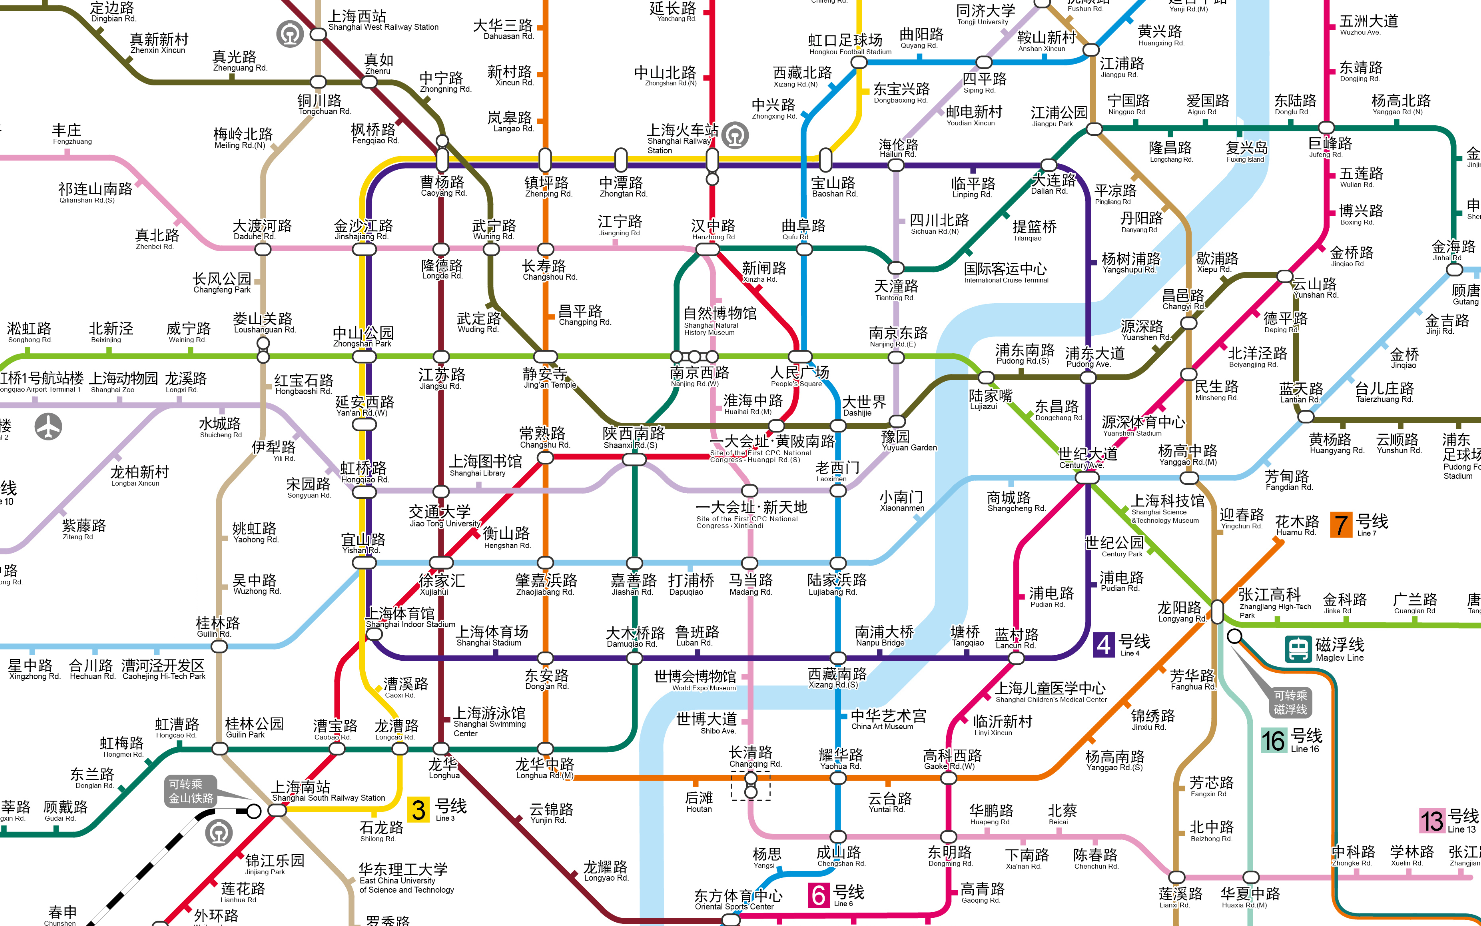
\includegraphics[scale=0.3]{img/C10/10-5/1.png}
	\caption{上海地铁线路图}
\end{figure}

在网络中,求两个不同顶点之间的所有路径中,边的权值之和最小的那一条路径,这条路径就是两点之间的最短路径。其中最短路径的第一个顶点称为源点(source),最后一个顶点为终点(destination)。\\

图的最短路径问题分为2种类型:

\begin{enumerate}
	\item 单源最短路径:从某固定源点出发,求到所有其它顶点的最短路径。
	\item 多源最短路径:求任意两顶点间的最短路径。
\end{enumerate}

\vspace{0.5cm}

\subsection{无权图的单源最短路径算法(SSSP, Single-Source Shortest Path)}

无权图的单源最短路径算法可以按照递增(非递减)的顺序找出到各个顶点的最短路,算法类似广度优先遍历。\\

例如在一个无权图中,以顶点3作为源点,离源点距离为1的顶点有1和6,距离为2的顶点有2和4,距离为3的顶点有5和7。

\begin{figure}[H]
	\centering
	\begin{tikzpicture}
		\begin{scope}[every node/.style={circle,thick,draw}]
			\node (1) at (-1.5,2) {1};
			\node (2) at (1.5,2) {2};
			\node (3) at (-4,0) {3};
			\node (4) at (0,0) {4};
			\node (5) at (4,0) {5};
			\node (6) at (-1.5,-2) {6};
			\node (7) at (1.5,-2) {7};
		\end{scope}

		\begin{scope}[>={Stealth[black]},
			every node/.style={},
			every edge/.style={draw=black,very thick}]
			\path [->] (1) edge node {} (2);
			\path [->] (1) edge node {} (4);
			\path [->] (2) edge node {} (4);
			\path [->] (2) edge node {} (5);
			\path [->] (3) edge node {} (1);
			\path [->] (3) edge node {} (6);
			\path [->] (4) edge node {} (3);
			\path [->] (4) edge node {} (5);
			\path [->] (4) edge node {} (6);
			\path [->] (4) edge node {} (7);
			\path [->] (5) edge node {} (7);
			\path [->] (7) edge node {} (6);
		\end{scope}
	\end{tikzpicture}
\end{figure}

无权图的单元最短路径算法中,dist[v]存储从源点S到v的最短路径,初始化源点dist[S]的距离为0,path[v]表示达到顶点路径v上一个经过的顶点。

\begin{table}[H]
	\centering
	\setlength{\tabcolsep}{5mm}{
		\begin{tabular}{|c|c|c|c|c|c|c|c|}
			\hline
			\textbf{顶点} & \textbf{1} & \textbf{2} & \textbf{3} & \textbf{4} & \textbf{5} & \textbf{6} & \textbf{7} \\
			\hline
			\textbf{dist} & 1          & 2          & 0          & 2          & 3          & 1          & 3          \\
			\hline
			\textbf{path} & 3          & 1          & -1         & 1          & 2          & 3          & 4          \\
			\hline
		\end{tabular}
	}
	\caption{数组VS链表}
\end{table}

\begin{algorithm}[H]
	\caption{无权图的单源最短路径}
	\begin{algorithmic}[1]
		\Procedure{unweightedSSSP}{Vertex S}
		\State enqueue(Q, S)
		\While {!isEmpty(Q)}
		\State V = dequeue(Q)
		\For {v in V}
		\If {dist[v] == -1}
		\State dist[v] = dist[V] + 1
		\State path[v] = V
		\State enqueue(Q, v)
		\EndIf
		\EndFor
		\EndWhile
		\EndProcedure
	\end{algorithmic}
\end{algorithm}

\vspace{0.5cm}

\subsection{有权图的单源最短路径算法}

有权图的最短路径不一定是经过顶点树最少的路。如果图中存在负值圈(negative-cost cycle)的话会导致算法失效,因为沿着回路走无穷多次,花销是负无穷。

\begin{figure}[H]
	\centering
	\begin{tikzpicture}
		\begin{scope}[every node/.style={circle,thick,draw}]
			\node (1) at (-1.5,2) {1};
			\node (2) at (1.5,2) {2};
			\node (3) at (-4,0) {3};
			\node (4) at (0,0) {4};
			\node (5) at (4,0) {5};
			\node (6) at (-1.5,-2) {6};
			\node (7) at (1.5,-2) {7};
		\end{scope}

		\begin{scope}[>={Stealth[black]},
			every node/.style={fill=white,circle},
			every edge/.style={draw=black,very thick}]
			\path [->] (1) edge node {2} (2);
			\path [->] (1) edge node {1} (4);
			\path [->, red] (4) edge node {3} (2);
			\path [->, red] (2) edge node {-10} (5);
			\path [->] (3) edge node {4} (1);
			\path [->] (3) edge node {5} (6);
			\path [->] (4) edge node {2} (3);
			\path [->, red] (5) edge node {2} (4);
			\path [->] (4) edge node {8} (6);
			\path [->] (4) edge node {4} (7);
			\path [->] (5) edge node {6} (7);
			\path [->] (7) edge node {1} (6);
		\end{scope}
	\end{tikzpicture}
	\caption{负值圈}
\end{figure}

带权图的单源最短路径可以通过迪杰斯特拉(Dijkstra)算法解决。\\

特斯拉?什么鬼?\\

迪杰斯特拉算法的本质是不断刷新起点与其他各个顶点之间的距离表。Dijkstra算法采用了贪心的思想,每次都未收录的顶点中选取dist值最小的收录。每当收录一个顶点时,可能会影响另外一个顶点的dist值。

\vspace{-0.5cm}

$$
	dist[w] = min\{dist[w], dist[v] + weight_{<v, w>}\}
$$

例如计算从源点A到其它各顶点的最短路径。

\begin{figure}[H]
	\centering
	\begin{tikzpicture}
		\begin{scope}[every node/.style={circle,thick,draw}]
			\node (A) at (-3,2.5) {A};
			\node (B) at (-4,0) {B};
			\node (C) at (0,3) {C};
			\node (D) at (0,0) {D};
			\node (E) at (-1.5,-2.5) {E};
			\node (F) at (2,-1) {F};
			\node (G) at (3,-3) {G};
		\end{scope}

		\begin{scope}[>={Stealth[black]},
			every node/.style={fill=white,circle},
			every edge/.style={draw=black,very thick}]
			\path [-] (A) edge node {5} (B);
			\path [-] (A) edge node {2} (C);
			\path [-] (B) edge node {1} (D);
			\path [-] (B) edge node {6} (E);
			\path [-] (C) edge node {6} (D);
			\path [-] (C) edge node {8} (F);
			\path [-] (E) edge node {1} (D);
			\path [-] (E) edge node {7} (G);
			\path [-] (F) edge node {3} (G);
		\end{scope}
	\end{tikzpicture}
\end{figure}

第1步:创建距离表。其中表中key是顶点名称,value是源点A到对应顶点的已知最短距离。一开始并不知道最短路径是多少,因此value都为$ \infty $。

\begin{table}[H]
	\centering
	\setlength{\tabcolsep}{5mm}{
		\begin{tabular}{|c|c|c|c|c|c|}
			\hline
			\textbf{B} & \textbf{C} & \textbf{D} & \textbf{E} & \textbf{F} & \textbf{G} \\
			\hline
			$ \infty $ & $ \infty $ & $ \infty $ & $ \infty $ & $ \infty $ & $ \infty $ \\
			\hline
		\end{tabular}
	}
\end{table}

第2步:找到源点A的邻接点B和C,从A到B的距离是5,从A到C的距离是2。

\begin{table}[H]
	\centering
	\setlength{\tabcolsep}{5mm}{
		\begin{tabular}{|c|c|c|c|c|c|}
			\hline
			\textbf{B}         & \textbf{C}         & \textbf{D} & \textbf{E} & \textbf{F} & \textbf{G} \\
			\hline
			\textcolor{red}{5} & \textcolor{red}{2} & $ \infty $ & $ \infty $ & $ \infty $ & $ \infty $ \\
			\hline
		\end{tabular}
	}
\end{table}

第3步:从距离表中找到从A出发距离最短的顶点,也就是顶点C。找到顶点C的邻接点D和F(A已经遍历过不需要考虑)。从C到D的距离是6,所以从A到D的距离是2 + 6 = 8;从C到F的距离是8,所以从A到F的距离是2 + 8 = 10。

\begin{table}[H]
	\centering
	\setlength{\tabcolsep}{5mm}{
		\begin{tabular}{|c|c|c|c|c|c|}
			\hline
			\textbf{B} & \textbf{C} & \textbf{D}         & \textbf{E} & \textbf{F}          & \textbf{G} \\
			\hline
			5          & 2          & \textcolor{red}{8} & $ \infty $ & \textcolor{red}{10} & $ \infty $ \\
			\hline
		\end{tabular}
	}
\end{table}

第4步:从距离表中找到从A出发距离最短的顶点(C已经遍历过不需要考虑),也就是顶点B。找到顶点B的邻接点D和E(A已经遍历过不需要考虑)。从B到D的距离是1,所以从A到D的距离是5 + 1 = 6,小于距离表中的8;从B到E的距离是6,所以从A到E的距离是5 + 6 = 11。

\begin{table}[H]
	\centering
	\setlength{\tabcolsep}{5mm}{
		\begin{tabular}{|c|c|c|c|c|c|}
			\hline
			\textbf{B} & \textbf{C} & \textbf{D}         & \textbf{E}          & \textbf{F} & \textbf{G} \\
			\hline
			5          & 2          & \textcolor{red}{6} & \textcolor{red}{11} & 10         & $ \infty $ \\
			\hline
		\end{tabular}
	}
\end{table}

第5步:从距离表中找到从A出发距离最短的顶点(B和C不用考虑),也就是顶点D。找到顶点D的邻接点E和F。从D到E的距离是1,所以从A到E的距离是6 + 1 = 7,小于距离表中的11;从D到F的距离是2,所以从A到F的距离是6 + 2 = 8,小于距离表中的10。

\begin{table}[H]
	\centering
	\setlength{\tabcolsep}{5mm}{
		\begin{tabular}{|c|c|c|c|c|c|}
			\hline
			\textbf{B} & \textbf{C} & \textbf{D} & \textbf{E}         & \textbf{F}         & \textbf{G} \\
			\hline
			5          & 2          & 6          & \textcolor{red}{7} & \textcolor{red}{8} & $ \infty $ \\
			\hline
		\end{tabular}
	}
\end{table}

第6步:从距离表中找到从A出发距离最短的顶点,也就是顶点E。找到顶点E的邻接点G。从E到G的距离是7,所以从A到G的距离是7 + 7 = 14。

\begin{table}[H]
	\centering
	\setlength{\tabcolsep}{5mm}{
		\begin{tabular}{|c|c|c|c|c|c|}
			\hline
			\textbf{B} & \textbf{C} & \textbf{D} & \textbf{E} & \textbf{F} & \textbf{G}          \\
			\hline
			5          & 2          & 6          & 7          & 8          & \textcolor{red}{14} \\
			\hline
		\end{tabular}
	}
\end{table}

第7步:从距离表中找到从A出发距离最短的顶点,也就是顶点F。找到顶点F的邻接点G。从F到G的距离是3,所以从A到G的距离是8 + 3 = 11,小于距离表中的14。

\begin{table}[H]
	\centering
	\setlength{\tabcolsep}{5mm}{
		\begin{tabular}{|c|c|c|c|c|c|}
			\hline
			\textbf{B} & \textbf{C} & \textbf{D} & \textbf{E} & \textbf{F} & \textbf{G}          \\
			\hline
			5          & 2          & 6          & 7          & 8          & \textcolor{red}{11} \\
			\hline
		\end{tabular}
	}
\end{table}

最终,距离表中存储的是从源点A到所有顶点的最短距离。\\

\subsection{多源最短路径算法}

如何能够求出一个带权图中所有顶点两两之间的最短距离呢?\\

对了!刚刚学过了Dijkstra算法,可以对每个顶点都使用一次Dijkstra算法,这样就求出了所有顶点之间的最短距离。\\

这个思路确实可以实现,但是Dijkstra算法的代码逻辑比较复杂,有没有更简单的方法呢?\\

弗洛伊德(Floyd-Warshall)算法是专门用于寻找带权图中多源点之间的最短路径算法。Floyd算法的思想是,若想缩短两点间的距离,仅有一种方式,那就是通过第三顶点绕行。\\

假设$ D^k[i][j] $为路径$ \{i \rightarrow \{l \le k\} \rightarrow j\} $的最小长度。当$ D^{k-1} $已经完成,递推到$ D^k $时:

\begin{enumerate}
	\item 如果$ k \notin \text{最短路径}\{i \rightarrow \{l \le k\} \rightarrow j\} $,则$ D^k = D^{k-1} $。
	\item 如果$ k \in \text{最短路径}\{i \rightarrow \{l \le k\} \rightarrow j\} $,该路径必定由两段最短路径组成,则$ D^k[i][j] = D^{k-1}[i][k] + D^{k-1}[k][j] $。
\end{enumerate}

例如,小哼准备去一些城市旅游,有些城市之间有公路,有些城市之间则没有。为了节省经费以及方便计划旅程,小哼希望在出发之前直到任意两个城市之间的最短路程。\\

如果要让任意两点之间的路程变短,只能引入第三个点,并通过这个顶点中转才有可能缩短原来的路程。这个中转的顶点甚至有时候不只通过一个顶点,而是经过两个或更多点中转会更短。\\

当任意两点之间不允许经过第三个点中转时,这些城市之间的最短路径就是邻接矩阵的初始路径。\\

\begin{figure}[H]
	\centering
	\begin{tikzpicture}
		\draw (0,0) circle(0.5) node{A};
		\draw (4,0) circle(0.5) node{B};
		\draw (4,4) circle(0.5) node{C};
		\draw (0,4) circle(0.5) node{D};

		\draw[->] (0.5,0) -- (2,0) node[below]{2} -- (3.5,0);
		\draw[->] (0.4,0.25) to[bend right] (3.75,3.6);
		\draw (3,1.5) node{6};
		\draw[->] (3.6,3.75) to[bend right] (0.25,0.4);
		\draw (1,2.5) node{7};
		\draw[->] (0,0.5) -- (0,2) node[left]{4} -- (0,3.5);
		\draw[->] (4,0.5) -- (4,2) node[right]{3} -- (4,3.5);
		\draw[->] (3.5,4) -- (2,4) node[above]{1} -- (0.5,4);
		\draw[->] (-0.5,4) to[bend right] (-0.5,0);
		\draw (-1.5,2) node{5};
		\draw[->] (0,4.5) to[bend left] (4,4.5);
		\draw (2,5.5) node{12};
	\end{tikzpicture}
\end{figure}

\begin{table}[H]
	\centering
	\setlength{\tabcolsep}{5mm}{
		\begin{tabular}{|c|c|c|c|c|}
			\hline
			           & \textbf{A} & \textbf{B} & \textbf{C} & \textbf{D} \\
			\hline
			\textbf{A} & 0          & 2          & 6          & 4          \\
			\hline
			\textbf{B} & $ \infty $ & 0          & 3          & $ \infty $ \\
			\hline
			\textbf{C} & 7          & $ \infty $ & 0          & 1          \\
			\hline
			\textbf{D} & 5          & $ \infty $ & 12         & 0          \\
			\hline
		\end{tabular}
	}
\end{table}

在只允许经过1号顶点中转的情况下,任意两点之间的最短路程更新为:

\begin{table}[H]
	\centering
	\setlength{\tabcolsep}{5mm}{
		\begin{tabular}{|c|c|c|c|c|}
			\hline
			           & \textbf{A} & \textbf{B}         & \textbf{C}          & \textbf{D} \\
			\hline
			\textbf{A} & 0          & 2                  & 6                   & 4          \\
			\hline
			\textbf{B} & $ \infty $ & 0                  & 3                   & $ \infty $ \\
			\hline
			\textbf{C} & 7          & \textcolor{red}{9} & 0                   & 1          \\
			\hline
			\textbf{D} & 5          & \textcolor{red}{7} & \textcolor{red}{11} & 0          \\
			\hline
		\end{tabular}
	}
\end{table}

在只允许经过1号和2号顶点中转的情况下,任意两点之间的最短路程更新为:

\begin{table}[H]
	\centering
	\setlength{\tabcolsep}{5mm}{
		\begin{tabular}{|c|c|c|c|c|}
			\hline
			           & \textbf{A} & \textbf{B} & \textbf{C}          & \textbf{D} \\
			\hline
			\textbf{A} & 0          & 2          & \textcolor{red}{5}  & 4          \\
			\hline
			\textbf{B} & $ \infty $ & 0          & 3                   & $ \infty $ \\
			\hline
			\textbf{C} & 7          & 9          & 0                   & 1          \\
			\hline
			\textbf{D} & 5          & 7          & \textcolor{red}{10} & 0          \\
			\hline
		\end{tabular}
	}
\end{table}

在只允许经过1号、2号和3号顶点中转的情况下,任意两点之间的最短路程更新为:

\begin{table}[H]
	\centering
	\setlength{\tabcolsep}{5mm}{
		\begin{tabular}{|c|c|c|c|c|}
			\hline
			           & \textbf{A}          & \textbf{B} & \textbf{C} & \textbf{D}         \\
			\hline
			\textbf{A} & 0                   & 2          & 5          & 4                  \\
			\hline
			\textbf{B} & \textcolor{red}{10} & 0          & 3          & \textcolor{red}{4} \\
			\hline
			\textbf{C} & 7                   & 9          & 0          & 1                  \\
			\hline
			\textbf{D} & 5                   & 7          & 10         & 0                  \\
			\hline
		\end{tabular}
	}
\end{table}

最后允许通过所有顶点作为中转,任意两点之间的最短路程更新为:

\begin{table}[H]
	\centering
	\setlength{\tabcolsep}{5mm}{
		\begin{tabular}{|c|c|c|c|c|}
			\hline
			           & \textbf{A}         & \textbf{B}         & \textbf{C} & \textbf{D} \\
			\hline
			\textbf{A} & 0                  & 2                  & 5          & 4          \\
			\hline
			\textbf{B} & \textcolor{red}{9} & 0                  & 3          & 4          \\
			\hline
			\textbf{C} & \textcolor{red}{6} & \textcolor{red}{8} & 0          & 1          \\
			\hline
			\textbf{D} & 5                  & 7                  & 10         & 0          \\
			\hline
		\end{tabular}
	}
\end{table}

\mybox{Floyd最短路径}

\begin{lstlisting}[language=C]
void floyd(Graph *g, int dist[MAX][MAX]) {
    // 最短路径矩阵初始化为图的邻接矩阵
    for(int i = 0; i < g->vertexNum; i++) {
        for(int j = 0; j < g->vertexNum; j++) {
            dist[i][j] = g->weight[i][j];
        }
    }

    // Floyd算法
    for(int k = 0; k < g->vertexNum; k++) {
        for(int i = 0; i < g->vertexNum; i++) {
            for(int j = 0; j < g->vertexNum; j++) {
                if(dist[i][k] + dist[k][j] < dist[i][j]) {
                    dist[i][j] = dist[i][k] + dist[k][j];
                }
            }
        }
    }
}
\end{lstlisting}

\newpage

\section{最小生成树}

\subsection{最小生成树(MST, Mininum Spanning Tree)}

所谓最小生成树,就是一个图的极小连通子图,它包含原图的所有顶点,并且所有边的权值之和尽可能小。\\

最小生成树需要满足3个条件:

\begin{enumerate}
	\item 是一棵树:树不能有回路,并且$ |V| $个顶点一定有$ |V| - 1 $条边。

	\item 是生成树:包含原图的全部顶点,树的$ |V| - 1 $条边都必须在图里,并且如果向生成树中任意加一条边都一定构成回路。

	\item 边的权重和最小。
\end{enumerate}

如果最小生成树存在,那么图一定连通,反之亦然。\\

例如一个带权图,蓝色边可以把所有顶点连接起来,又保证边的权值和最小。

\begin{figure}[H]
	\centering
	\begin{tikzpicture}
		\begin{scope}[every node/.style={circle,thick,draw}]
			\node (A) at (-1.5,2) {A};
			\node (B) at (1.5,2) {B};
			\node (C) at (-4,0) {C};
			\node (D) at (0,0) {D};
			\node (E) at (4,0) {E};
			\node (F) at (-1.5,-2) {F};
		\end{scope}

		\begin{scope}[>={Stealth[black]},
			every node/.style={fill=white,circle},
			every edge/.style={draw=black,very thick}]
			\path [->] (B) edge node {7} (E);
			\path [->] (C) edge node {5} (D);
			\path [->] (F) edge node {9} (E);
		\end{scope}

		\begin{scope}[>={Stealth[blue]},
			every node/.style={fill=white,circle},
			every edge/.style={draw=blue,very thick}]
			\path [->] (A) edge node {4} (B);
			\path [->] (A) edge node {3} (C);
			\path [->] (A) edge node {1} (D);
			\path [->] (D) edge node {2} (F);
			\path [->] (D) edge node {3} (E);
		\end{scope}
	\end{tikzpicture}
\end{figure}

\begin{figure}[H]
	\centering
	\begin{tikzpicture}[
			level distance=1.5cm,
			level 1/.style={sibling distance=2cm},
			level 2/.style={sibling distance=1.5cm},
			level 3/.style={sibling distance=1cm}
		]
		\node[circle,draw] {A}
		child {node[circle,draw] {B}}
		child {node[circle,draw] {C}}
		child {
				node[circle,draw] {D}
				child {node[circle,draw] {E}}
				child {node[circle,draw] {F}}
			};
	\end{tikzpicture}
	\caption{最小生成树}
\end{figure}

图的最小生成树不是唯一的,同一个图有可能对应多个最小生成树。\\

最小生成树在现实中很很多用处。假如要在若干个城市之间铺设铁路,而预算又是有限的,那么就需要寻找成本最低的铺设方式。城市之间的交通网就像一个连通图,其实并不需要在每两个城市之间都直接进行连接,只需要一个最小生成树,保证所有的城市都有铁路可以达到即可。\\

\subsection{Prim}

Prim算法是以图的顶点为基础,从一个初始顶点开始,寻找达到其它顶点权值最小的边,并把该顶点加入到已触达顶点的集合中。当全部顶点都加入到集合时,算法的工作就完成了。Prim算法的本质是基于贪心算法(greedy algorithm)。\\

Prim算法可以理解为让一棵小树长大,每次找能够向外生长的最小边。\\

例如使用Prim算法获得一个带权图的最小生成树:

\begin{figure}[H]
	\centering
	\begin{tikzpicture}
		\begin{scope}[every node/.style={circle,thick,draw}]
			\node (A) at (-1.5,2) {A};
			\node (B) at (1.5,2) {B};
			\node (C) at (-4,0) {C};
			\node (D) at (0,0) {D};
			\node (E) at (4,0) {E};
			\node (F) at (-1.5,-2) {F};
			\node (G) at (1.5,-2) {G};
		\end{scope}

		\begin{scope}[>={Stealth[black]},
			every node/.style={fill=white,circle},
			every edge/.style={draw=black,very thick}]
			\path [-] (A) edge node {2} (B);
			\path [-] (A) edge node {1} (D);
			\path [-] (B) edge node {3} (D);
			\path [-] (B) edge node {10} (E);
			\path [-] (C) edge node {4} (A);
			\path [-] (C) edge node {5} (F);
			\path [-] (D) edge node {2} (C);
			\path [-] (D) edge node {7} (E);
			\path [-] (D) edge node {8} (F);
			\path [-] (D) edge node {4} (G);
			\path [-] (E) edge node {6} (G);
			\path [-] (G) edge node {1} (F);
		\end{scope}
	\end{tikzpicture}
\end{figure}

\begin{figure}[H]
	\centering
	\begin{tikzpicture}
		\begin{scope}[every node/.style={circle,thick,draw}]
			\node (A) at (-1.5,2) {\textcolor{red}{A}};
			\node (B) at (1.5,2) {B};
			\node (C) at (-4,0) {C};
			\node (D) at (0,0) {D};
			\node (E) at (4,0) {E};
			\node (F) at (-1.5,-2) {F};
			\node (G) at (1.5,-2) {G};
		\end{scope}

		\begin{scope}[>={Stealth[black]},
			every node/.style={fill=white,circle},
			every edge/.style={draw=black,very thick}]
			\path [-] (A) edge node {2} (B);
			\path [-] (A) edge node {1} (D);
			\path [-] (B) edge node {3} (D);
			\path [-] (B) edge node {10} (E);
			\path [-] (C) edge node {4} (A);
			\path [-] (C) edge node {5} (F);
			\path [-] (D) edge node {2} (C);
			\path [-] (D) edge node {7} (E);
			\path [-] (D) edge node {8} (F);
			\path [-] (D) edge node {4} (G);
			\path [-] (E) edge node {6} (G);
			\path [-] (G) edge node {1} (F);
		\end{scope}
	\end{tikzpicture}
\end{figure}

\begin{figure}[H]
	\centering
	\begin{tikzpicture}
		\begin{scope}[every node/.style={circle,thick,draw}]
			\node (A) at (-1.5,2) {\textcolor{red}{A}};
			\node (B) at (1.5,2) {B};
			\node (C) at (-4,0) {C};
			\node (D) at (0,0) {\textcolor{red}{D}};
			\node (E) at (4,0) {E};
			\node (F) at (-1.5,-2) {F};
			\node (G) at (1.5,-2) {G};
		\end{scope}

		\begin{scope}[>={Stealth[black]},
			every node/.style={fill=white,circle},
			every edge/.style={draw=black,very thick}]
			\path [-] (A) edge node {2} (B);
			\path [-] (B) edge node {3} (D);
			\path [-] (B) edge node {10} (E);
			\path [-] (C) edge node {4} (A);
			\path [-] (C) edge node {5} (F);
			\path [-] (D) edge node {2} (C);
			\path [-] (D) edge node {7} (E);
			\path [-] (D) edge node {8} (F);
			\path [-] (D) edge node {4} (G);
			\path [-] (E) edge node {6} (G);
			\path [-] (G) edge node {1} (F);
		\end{scope}

		\begin{scope}[>={Stealth[red]},
			every node/.style={fill=white,circle},
			every edge/.style={draw=red,very thick}]
			\path [-] (A) edge node {1} (D);
		\end{scope}
	\end{tikzpicture}
\end{figure}

\begin{figure}[H]
	\centering
	\begin{tikzpicture}
		\begin{scope}[every node/.style={circle,thick,draw}]
			\node (A) at (-1.5,2) {\textcolor{red}{A}};
			\node (B) at (1.5,2) {\textcolor{red}{B}};
			\node (C) at (-4,0) {C};
			\node (D) at (0,0) {\textcolor{red}{D}};
			\node (E) at (4,0) {E};
			\node (F) at (-1.5,-2) {F};
			\node (G) at (1.5,-2) {G};
		\end{scope}

		\begin{scope}[>={Stealth[black]},
			every node/.style={fill=white,circle},
			every edge/.style={draw=black,very thick}]
			\path [-] (B) edge node {3} (D);
			\path [-] (B) edge node {10} (E);
			\path [-] (C) edge node {4} (A);
			\path [-] (C) edge node {5} (F);
			\path [-] (D) edge node {2} (C);
			\path [-] (D) edge node {7} (E);
			\path [-] (D) edge node {8} (F);
			\path [-] (D) edge node {4} (G);
			\path [-] (E) edge node {6} (G);
			\path [-] (G) edge node {1} (F);
		\end{scope}

		\begin{scope}[>={Stealth[red]},
			every node/.style={fill=white,circle},
			every edge/.style={draw=red,very thick}]
			\path [-] (A) edge node {1} (D);
			\path [-] (A) edge node {2} (B);
		\end{scope}
	\end{tikzpicture}
\end{figure}

\begin{figure}[H]
	\centering
	\begin{tikzpicture}
		\begin{scope}[every node/.style={circle,thick,draw}]
			\node (A) at (-1.5,2) {\textcolor{red}{A}};
			\node (B) at (1.5,2) {\textcolor{red}{B}};
			\node (C) at (-4,0) {\textcolor{red}{C}};
			\node (D) at (0,0) {\textcolor{red}{D}};
			\node (E) at (4,0) {E};
			\node (F) at (-1.5,-2) {F};
			\node (G) at (1.5,-2) {G};
		\end{scope}

		\begin{scope}[>={Stealth[black]},
			every node/.style={fill=white,circle},
			every edge/.style={draw=black,very thick}]
			\path [-] (B) edge node {3} (D);
			\path [-] (B) edge node {10} (E);
			\path [-] (C) edge node {4} (A);
			\path [-] (C) edge node {5} (F);
			\path [-] (D) edge node {7} (E);
			\path [-] (D) edge node {8} (F);
			\path [-] (D) edge node {4} (G);
			\path [-] (E) edge node {6} (G);
			\path [-] (G) edge node {1} (F);
		\end{scope}

		\begin{scope}[>={Stealth[red]},
			every node/.style={fill=white,circle},
			every edge/.style={draw=red,very thick}]
			\path [-] (A) edge node {1} (D);
			\path [-] (A) edge node {2} (B);
			\path [-] (D) edge node {2} (C);
		\end{scope}
	\end{tikzpicture}
\end{figure}

\begin{figure}[H]
	\centering
	\begin{tikzpicture}
		\begin{scope}[every node/.style={circle,thick,draw}]
			\node (A) at (-1.5,2) {\textcolor{red}{A}};
			\node (B) at (1.5,2) {\textcolor{red}{B}};
			\node (C) at (-4,0) {\textcolor{red}{C}};
			\node (D) at (0,0) {\textcolor{red}{D}};
			\node (E) at (4,0) {E};
			\node (F) at (-1.5,-2) {F};
			\node (G) at (1.5,-2) {\textcolor{red}{G}};
		\end{scope}

		\begin{scope}[>={Stealth[black]},
			every node/.style={fill=white,circle},
			every edge/.style={draw=black,very thick}]
			\path [-] (B) edge node {3} (D);
			\path [-] (B) edge node {10} (E);
			\path [-] (C) edge node {4} (A);
			\path [-] (C) edge node {5} (F);
			\path [-] (D) edge node {7} (E);
			\path [-] (D) edge node {8} (F);
			\path [-] (E) edge node {6} (G);
			\path [-] (G) edge node {1} (F);
		\end{scope}

		\begin{scope}[>={Stealth[red]},
			every node/.style={fill=white,circle},
			every edge/.style={draw=red,very thick}]
			\path [-] (A) edge node {1} (D);
			\path [-] (A) edge node {2} (B);
			\path [-] (D) edge node {2} (C);
			\path [-] (D) edge node {4} (G);
		\end{scope}
	\end{tikzpicture}
\end{figure}

\begin{figure}[H]
	\centering
	\begin{tikzpicture}
		\begin{scope}[every node/.style={circle,thick,draw}]
			\node (A) at (-1.5,2) {\textcolor{red}{A}};
			\node (B) at (1.5,2) {\textcolor{red}{B}};
			\node (C) at (-4,0) {\textcolor{red}{C}};
			\node (D) at (0,0) {\textcolor{red}{D}};
			\node (E) at (4,0) {E};
			\node (F) at (-1.5,-2) {\textcolor{red}{F}};
			\node (G) at (1.5,-2) {\textcolor{red}{G}};
		\end{scope}

		\begin{scope}[>={Stealth[black]},
			every node/.style={fill=white,circle},
			every edge/.style={draw=black,very thick}]
			\path [-] (B) edge node {3} (D);
			\path [-] (B) edge node {10} (E);
			\path [-] (C) edge node {4} (A);
			\path [-] (C) edge node {5} (F);
			\path [-] (D) edge node {7} (E);
			\path [-] (D) edge node {8} (F);
			\path [-] (E) edge node {6} (G);
		\end{scope}

		\begin{scope}[>={Stealth[red]},
			every node/.style={fill=white,circle},
			every edge/.style={draw=red,very thick}]
			\path [-] (A) edge node {1} (D);
			\path [-] (A) edge node {2} (B);
			\path [-] (D) edge node {2} (C);
			\path [-] (D) edge node {4} (G);
			\path [-] (G) edge node {1} (F);
		\end{scope}
	\end{tikzpicture}
\end{figure}

\begin{figure}[H]
	\centering
	\begin{tikzpicture}
		\begin{scope}[every node/.style={circle,thick,draw}]
			\node (A) at (-1.5,2) {\textcolor{red}{A}};
			\node (B) at (1.5,2) {\textcolor{red}{B}};
			\node (C) at (-4,0) {\textcolor{red}{C}};
			\node (D) at (0,0) {\textcolor{red}{D}};
			\node (E) at (4,0) {\textcolor{red}{E}};
			\node (F) at (-1.5,-2) {\textcolor{red}{F}};
			\node (G) at (1.5,-2) {\textcolor{red}{G}};
		\end{scope}

		\begin{scope}[>={Stealth[black]},
			every node/.style={fill=white,circle},
			every edge/.style={draw=black,very thick}]
			\path [-] (B) edge node {3} (D);
			\path [-] (B) edge node {10} (E);
			\path [-] (C) edge node {4} (A);
			\path [-] (C) edge node {5} (F);
			\path [-] (D) edge node {7} (E);
			\path [-] (D) edge node {8} (F);
		\end{scope}

		\begin{scope}[>={Stealth[red]},
			every node/.style={fill=white,circle},
			every edge/.style={draw=red,very thick}]
			\path [-] (A) edge node {1} (D);
			\path [-] (A) edge node {2} (B);
			\path [-] (D) edge node {2} (C);
			\path [-] (D) edge node {4} (G);
			\path [-] (G) edge node {1} (F);
			\path [-] (E) edge node {6} (G);
		\end{scope}
	\end{tikzpicture}
\end{figure}

\vspace{0.5cm}

\subsection{Kruskal}

与Prim算法不同,Prim算法是以顶点为关键来获得最小生成树的,而Kruskal算法是以边为关键获得最小生成树的。\\

Kruskal算法可以理解为将森林合并成树,每次在图中找权值最小的边收录。\\

例如使用Kruskal算法获得一个带权图的最小生成树:

\begin{figure}[H]
	\centering
	\begin{tikzpicture}
		\begin{scope}[every node/.style={circle,thick,draw}]
			\node (A) at (-1.5,2) {\textcolor{red}{A}};
			\node (B) at (1.5,2) {B};
			\node (C) at (-4,0) {C};
			\node (D) at (0,0) {\textcolor{red}{D}};
			\node (E) at (4,0) {E};
			\node (F) at (-1.5,-2) {F};
			\node (G) at (1.5,-2) {G};
		\end{scope}

		\begin{scope}[>={Stealth[black]},
			every node/.style={fill=white,circle},
			every edge/.style={draw=black,very thick}]
			\path [-] (A) edge node {2} (B);
			\path [-] (B) edge node {3} (D);
			\path [-] (B) edge node {10} (E);
			\path [-] (C) edge node {4} (A);
			\path [-] (C) edge node {5} (F);
			\path [-] (D) edge node {2} (C);
			\path [-] (D) edge node {7} (E);
			\path [-] (D) edge node {8} (F);
			\path [-] (D) edge node {4} (G);
			\path [-] (E) edge node {6} (G);
			\path [-] (G) edge node {1} (F);
		\end{scope}

		\begin{scope}[>={Stealth[red]},
			every node/.style={fill=white,circle},
			every edge/.style={draw=red,very thick}]
			\path [-] (A) edge node {1} (D);
		\end{scope}
	\end{tikzpicture}
\end{figure}

\begin{figure}[H]
	\centering
	\begin{tikzpicture}
		\begin{scope}[every node/.style={circle,thick,draw}]
			\node (A) at (-1.5,2) {\textcolor{red}{A}};
			\node (B) at (1.5,2) {B};
			\node (C) at (-4,0) {C};
			\node (D) at (0,0) {\textcolor{red}{D}};
			\node (E) at (4,0) {E};
			\node (F) at (-1.5,-2) {\textcolor{red}{F}};
			\node (G) at (1.5,-2) {\textcolor{red}{G}};
		\end{scope}

		\begin{scope}[>={Stealth[black]},
			every node/.style={fill=white,circle},
			every edge/.style={draw=black,very thick}]
			\path [-] (A) edge node {2} (B);
			\path [-] (B) edge node {3} (D);
			\path [-] (B) edge node {10} (E);
			\path [-] (C) edge node {4} (A);
			\path [-] (C) edge node {5} (F);
			\path [-] (D) edge node {2} (C);
			\path [-] (D) edge node {7} (E);
			\path [-] (D) edge node {8} (F);
			\path [-] (D) edge node {4} (G);
			\path [-] (E) edge node {6} (G);
		\end{scope}

		\begin{scope}[>={Stealth[red]},
			every node/.style={fill=white,circle},
			every edge/.style={draw=red,very thick}]
			\path [-] (A) edge node {1} (D);
			\path [-] (G) edge node {1} (F);
		\end{scope}
	\end{tikzpicture}
\end{figure}

\begin{figure}[H]
	\centering
	\begin{tikzpicture}
		\begin{scope}[every node/.style={circle,thick,draw}]
			\node (A) at (-1.5,2) {\textcolor{red}{A}};
			\node (B) at (1.5,2) {B};
			\node (C) at (-4,0) {\textcolor{red}{C}};
			\node (D) at (0,0) {\textcolor{red}{D}};
			\node (E) at (4,0) {E};
			\node (F) at (-1.5,-2) {\textcolor{red}{F}};
			\node (G) at (1.5,-2) {\textcolor{red}{G}};
		\end{scope}

		\begin{scope}[>={Stealth[black]},
			every node/.style={fill=white,circle},
			every edge/.style={draw=black,very thick}]
			\path [-] (A) edge node {2} (B);
			\path [-] (B) edge node {3} (D);
			\path [-] (B) edge node {10} (E);
			\path [-] (C) edge node {4} (A);
			\path [-] (C) edge node {5} (F);
			\path [-] (D) edge node {7} (E);
			\path [-] (D) edge node {8} (F);
			\path [-] (D) edge node {4} (G);
			\path [-] (E) edge node {6} (G);
		\end{scope}

		\begin{scope}[>={Stealth[red]},
			every node/.style={fill=white,circle},
			every edge/.style={draw=red,very thick}]
			\path [-] (A) edge node {1} (D);
			\path [-] (G) edge node {1} (F);
			\path [-] (D) edge node {2} (C);
		\end{scope}
	\end{tikzpicture}
\end{figure}

\begin{figure}[H]
	\centering
	\begin{tikzpicture}
		\begin{scope}[every node/.style={circle,thick,draw}]
			\node (A) at (-1.5,2) {\textcolor{red}{A}};
			\node (B) at (1.5,2) {\textcolor{red}{B}};
			\node (C) at (-4,0) {\textcolor{red}{C}};
			\node (D) at (0,0) {\textcolor{red}{D}};
			\node (E) at (4,0) {E};
			\node (F) at (-1.5,-2) {\textcolor{red}{F}};
			\node (G) at (1.5,-2) {\textcolor{red}{G}};
		\end{scope}

		\begin{scope}[>={Stealth[black]},
			every node/.style={fill=white,circle},
			every edge/.style={draw=black,very thick}]
			\path [-] (B) edge node {3} (D);
			\path [-] (B) edge node {10} (E);
			\path [-] (C) edge node {4} (A);
			\path [-] (C) edge node {5} (F);
			\path [-] (D) edge node {7} (E);
			\path [-] (D) edge node {8} (F);
			\path [-] (D) edge node {4} (G);
			\path [-] (E) edge node {6} (G);
		\end{scope}

		\begin{scope}[>={Stealth[red]},
			every node/.style={fill=white,circle},
			every edge/.style={draw=red,very thick}]
			\path [-] (A) edge node {1} (D);
			\path [-] (G) edge node {1} (F);
			\path [-] (D) edge node {2} (C);
			\path [-] (A) edge node {2} (B);
		\end{scope}
	\end{tikzpicture}
\end{figure}

\begin{figure}[H]
	\centering
	\begin{tikzpicture}
		\begin{scope}[every node/.style={circle,thick,draw}]
			\node (A) at (-1.5,2) {\textcolor{red}{A}};
			\node (B) at (1.5,2) {\textcolor{red}{B}};
			\node (C) at (-4,0) {\textcolor{red}{C}};
			\node (D) at (0,0) {\textcolor{red}{D}};
			\node (E) at (4,0) {E};
			\node (F) at (-1.5,-2) {\textcolor{red}{F}};
			\node (G) at (1.5,-2) {\textcolor{red}{G}};
		\end{scope}

		\begin{scope}[>={Stealth[black]},
			every node/.style={fill=white,circle},
			every edge/.style={draw=black,very thick}]
			\path [-] (B) edge node {3} (D);
			\path [-] (B) edge node {10} (E);
			\path [-] (C) edge node {4} (A);
			\path [-] (C) edge node {5} (F);
			\path [-] (D) edge node {7} (E);
			\path [-] (D) edge node {8} (F);
			\path [-] (E) edge node {6} (G);
		\end{scope}

		\begin{scope}[>={Stealth[red]},
			every node/.style={fill=white,circle},
			every edge/.style={draw=red,very thick}]
			\path [-] (A) edge node {1} (D);
			\path [-] (G) edge node {1} (F);
			\path [-] (D) edge node {2} (C);
			\path [-] (A) edge node {2} (B);
			\path [-] (D) edge node {4} (G);
		\end{scope}
	\end{tikzpicture}
\end{figure}

\begin{figure}[H]
	\centering
	\begin{tikzpicture}
		\begin{scope}[every node/.style={circle,thick,draw}]
			\node (A) at (-1.5,2) {\textcolor{red}{A}};
			\node (B) at (1.5,2) {\textcolor{red}{B}};
			\node (C) at (-4,0) {\textcolor{red}{C}};
			\node (D) at (0,0) {\textcolor{red}{D}};
			\node (E) at (4,0) {\textcolor{red}{E}};
			\node (F) at (-1.5,-2) {\textcolor{red}{F}};
			\node (G) at (1.5,-2) {\textcolor{red}{G}};
		\end{scope}

		\begin{scope}[>={Stealth[black]},
			every node/.style={fill=white,circle},
			every edge/.style={draw=black,very thick}]
			\path [-] (B) edge node {3} (D);
			\path [-] (B) edge node {10} (E);
			\path [-] (C) edge node {4} (A);
			\path [-] (C) edge node {5} (F);
			\path [-] (D) edge node {7} (E);
			\path [-] (D) edge node {8} (F);
		\end{scope}

		\begin{scope}[>={Stealth[red]},
			every node/.style={fill=white,circle},
			every edge/.style={draw=red,very thick}]
			\path [-] (A) edge node {1} (D);
			\path [-] (G) edge node {1} (F);
			\path [-] (D) edge node {2} (C);
			\path [-] (A) edge node {2} (B);
			\path [-] (D) edge node {4} (G);
			\path [-] (E) edge node {6} (G);
		\end{scope}
	\end{tikzpicture}
\end{figure}

\newpage

\section{拓扑排序}

\subsection{拓扑排序(Topological Sort)}

一项大的工程常被分为多个小的子工程,子工程之间可能存在一定的先后顺序,即某些子工程必须在其它的一些子工程完成后才能开始。在现代化管理中,有向图可以用来描述和分析一项工程的计划和实施过程,其中图的顶点表示活动,有向边表示活动之间的先后关系,这样的图称为AOV(Activity on Vertex)网。

\begin{figure}[H]
	\centering
	\begin{tikzpicture}
		\begin{scope}[every node/.style={circle,thick,draw}]
			\node (A) at (0,0) {A};
			\node (B) at (2,0) {B};
			\node (C) at (3.5,1.5) {C};
			\node (D) at (3.5,-1.5) {D};
			\node (E) at (5,0) {E};
			\node (F) at (7,0){F};
		\end{scope}

		\begin{scope}[>={Stealth[black]},
			every node/.style={},
			every edge/.style={draw=black,very thick}]
			\path [->] (A) edge node {} (B);
			\path [->] (B) edge node {} (C);
			\path [->] (B) edge node {} (D);
			\path [->] (C) edge node {} (E);
			\path [->] (B) edge node {} (E);
			\path [->] (D) edge node {} (E);
			\path [->] (E) edge node {} (F);
		\end{scope}
	\end{tikzpicture}
	\caption{AOV网}
\end{figure}

如果图中从顶点V到W有一条有向路径,则V一定排在W之前,满足此条件的顶点序列称为一个拓扑序。AOV网如果有合理的拓扑序,则必定是有向无环图(DAG, Directed Acyclic Graph)。\\

可以使用卡恩Kahn算法完成拓扑排序。假设列表$ L $用于存放拓扑排序的结果,把所有入度为0的顶点放入L中,然后把这些顶点从图中去掉。重复该操作,直到找不到入度为0的顶点。如果此时L中的元素个数和图的顶点总数相同,说明拓扑排序完成;如果此时L中的元素个数少于图的顶点总数,说明原图中存在环,无法进行拓扑排序。\\

例如对计算机专业课安排学习顺序:

\begin{table}[H]
	\centering
	\setlength{\tabcolsep}{5mm}{
		\begin{tabular}{|c|c|c|}
			\hline
			\textbf{课程代码} & \textbf{课程名称}    & \textbf{预修课程} \\
			\hline
			C1                & 程序设计基础         & 无                \\
			\hline
			C2                & 离散数学             & 无                \\
			\hline
			C3                & 数据结构             & C1、C2            \\
			\hline
			C4                & 微积分(一)         & 无                \\
			\hline
			C5                & 微积分(二)         & C4                \\
			\hline
			C6                & 线性代数             & C5                \\
			\hline
			C7                & 算法分析与设计       & C3                \\
			\hline
			C8                & 逻辑与计算机设计基础 & 无                \\
			\hline
			C9                & 计算机组成           & C8                \\
			\hline
			C10               & 操作系统             & C7、C9            \\
			\hline
			C11               & 编译原理             & C7、C9            \\
			\hline
			C12               & 数据库               & C7                \\
			\hline
			C13               & 计算理论             & C2                \\
			\hline
			C14               & 计算机网络           & C10               \\
			\hline
			C15               & 数值分析             & C6                \\
			\hline
		\end{tabular}
	}
	\caption{计算机专业课}
\end{table}

\begin{figure}[H]
	\centering
	\begin{tikzpicture}
		\begin{scope}[every node/.style={circle,thick,draw}]
			\node (C1) at (0,6) {C1};
			\node (C2) at (0,4) {C2};
			\node (C3) at (2,5) {C3};
			\node (C4) at (0,0) {C4};
			\node (C5) at (2,0) {C5};
			\node (C6) at (4,0) {C6};
			\node (C7) at (4,5) {C7};
			\node (C8) at (0,2) {C8};
			\node (C9) at (2,2) {C9};
			\node (C10) at (6,3) {C10};
			\node (C11) at (4.5,1.5) {C11};
			\node (C12) at (6,5) {C12};
			\node (C13) at (3,3.5) {C13};
			\node (C14) at (8,3) {C14};
			\node (C15) at (6,0) {C15};
		\end{scope}

		\begin{scope}[>={Stealth[black]},
			every node/.style={},
			every edge/.style={draw=black,very thick}]
			\path [->] (C1) edge node {} (C3);
			\path [->] (C2) edge node {} (C3);
			\path [->] (C2) edge node {} (C13);
			\path [->] (C3) edge node {} (C7);
			\path [->] (C7) edge node {} (C12);
			\path [->] (C7) edge node {} (C10);
			\path [->] (C7) edge node {} (C11);
			\path [->] (C8) edge node {} (C9);
			\path [->] (C9) edge node {} (C10);
			\path [->] (C9) edge node {} (C11);
			\path [->] (C4) edge node {} (C5);
			\path [->] (C5) edge node {} (C6);
			\path [->] (C6) edge node {} (C15);
			\path [->] (C10) edge node {} (C14);
		\end{scope}
	\end{tikzpicture}
	\caption{计算机专业课AOV网}
\end{figure}

\begin{figure}[H]
	\centering
	\begin{tikzpicture}
		\begin{scope}[every node/.style={circle,thick,draw}]
			\node (C3) at (2,5) {C3};
			\node (C5) at (2,0) {C5};
			\node (C6) at (4,0) {C6};
			\node (C7) at (4,5) {C7};
			\node (C9) at (2,2) {C9};
			\node (C10) at (6,3) {C10};
			\node (C11) at (4.5,1.5) {C11};
			\node (C12) at (6,5) {C12};
			\node (C13) at (3,3.5) {C13};
			\node (C14) at (8,3) {C14};
			\node (C15) at (6,0) {C15};
		\end{scope}

		\begin{scope}[>={Stealth[black]},
			every node/.style={},
			every edge/.style={draw=black,very thick}]
			\path [->] (C3) edge node {} (C7);
			\path [->] (C7) edge node {} (C12);
			\path [->] (C7) edge node {} (C10);
			\path [->] (C7) edge node {} (C11);
			\path [->] (C9) edge node {} (C10);
			\path [->] (C9) edge node {} (C11);
			\path [->] (C5) edge node {} (C6);
			\path [->] (C6) edge node {} (C15);
			\path [->] (C10) edge node {} (C14);
		\end{scope}
	\end{tikzpicture}
\end{figure}

\begin{table}[H]
	\centering
	\setlength{\tabcolsep}{5mm}{
		\begin{tabular}{|c|c|}
			\hline
			\textbf{学期}     & \textbf{课程}  \\
			\hline
			\textbf{第一学期} & C1、C2、C4、C8 \\
			\hline
		\end{tabular}
	}
	\caption{第一学期课程}
\end{table}

\begin{figure}[H]
	\centering
	\begin{tikzpicture}
		\begin{scope}[every node/.style={circle,thick,draw}]
			\node (C6) at (4,0) {C6};
			\node (C7) at (4,5) {C7};
			\node (C10) at (6,3) {C10};
			\node (C11) at (4.5,1.5) {C11};
			\node (C12) at (6,5) {C12};
			\node (C14) at (8,3) {C14};
			\node (C15) at (6,0) {C15};
		\end{scope}

		\begin{scope}[>={Stealth[black]},
			every node/.style={},
			every edge/.style={draw=black,very thick}]
			\path [->] (C7) edge node {} (C12);
			\path [->] (C7) edge node {} (C10);
			\path [->] (C7) edge node {} (C11);
			\path [->] (C6) edge node {} (C15);
			\path [->] (C10) edge node {} (C14);
		\end{scope}
	\end{tikzpicture}
\end{figure}

\begin{table}[H]
	\centering
	\setlength{\tabcolsep}{5mm}{
		\begin{tabular}{|c|c|}
			\hline
			\textbf{学期}     & \textbf{课程}   \\
			\hline
			\textbf{第一学期} & C1、C2、C4、C8  \\
			\hline
			\textbf{第二学期} & C3、C5、C9、C13 \\
			\hline
		\end{tabular}
	}
	\caption{第二学期课程}
\end{table}

\begin{figure}[H]
	\centering
	\begin{tikzpicture}
		\begin{scope}[every node/.style={circle,thick,draw}]
			\node (C10) at (6,3) {C10};
			\node (C11) at (4.5,1.5) {C11};
			\node (C12) at (6,5) {C12};
			\node (C14) at (8,3) {C14};
			\node (C15) at (6,0) {C15};
		\end{scope}

		\begin{scope}[>={Stealth[black]},
			every node/.style={},
			every edge/.style={draw=black,very thick}]
			\path [->] (C10) edge node {} (C14);
		\end{scope}
	\end{tikzpicture}
\end{figure}

\begin{table}[H]
	\centering
	\setlength{\tabcolsep}{5mm}{
		\begin{tabular}{|c|c|}
			\hline
			\textbf{学期}     & \textbf{课程}   \\
			\hline
			\textbf{第一学期} & C1、C2、C4、C8  \\
			\hline
			\textbf{第二学期} & C3、C5、C9、C13 \\
			\hline
			\textbf{第三学期} & C6、C7          \\
			\hline
		\end{tabular}
	}
	\caption{第三学期课程}
\end{table}

\begin{figure}[H]
	\centering
	\begin{tikzpicture}
		\begin{scope}[every node/.style={circle,thick,draw}]
			\node (C14) at (8,3) {C14};
		\end{scope}
	\end{tikzpicture}
\end{figure}

\begin{table}[H]
	\centering
	\setlength{\tabcolsep}{5mm}{
		\begin{tabular}{|c|c|}
			\hline
			\textbf{学期}     & \textbf{课程}      \\
			\hline
			\textbf{第一学期} & C1、C2、C4、C8     \\
			\hline
			\textbf{第二学期} & C3、C5、C9、C13    \\
			\hline
			\textbf{第三学期} & C6、C7             \\
			\hline
			\textbf{第四学期} & C10、C11、C12、C15 \\
			\hline
		\end{tabular}
	}
	\caption{第四学期课程}
\end{table}

\begin{table}[H]
	\centering
	\setlength{\tabcolsep}{5mm}{
		\begin{tabular}{|c|c|}
			\hline
			\textbf{学期}     & \textbf{课程}      \\
			\hline
			\textbf{第一学期} & C1、C2、C4、C8     \\
			\hline
			\textbf{第二学期} & C3、C5、C9、C13    \\
			\hline
			\textbf{第三学期} & C6、C7             \\
			\hline
			\textbf{第四学期} & C10、C11、C12、C15 \\
			\hline
			\textbf{第五学期} & C14                \\
			\hline
		\end{tabular}
	}
	\caption{第五学期课程}
\end{table}